% $Id: 
% ..............................................................................
%             M E N U E S  i n  V E R S C H I E D E N E N  C T - V A R I A N T E N
% ~~~~~~~~~~~~~~~~~~~~~~~~~~~~~~~~~~~~~~~~~~~~~~~~~~~~~~~~~~~~~~~~~~~~~~~~~~~~~~

\newpage
%\enlargethispage{1cm}
\hypertarget{appendix-menu-overview-CT1}{}
\section{CrypTool~1 Menus}
\label{s:appendix-menu-overview-CT1}

This appendix contains at the following page the complete menu tree of
CrypTool\index{CrypTool} version 1.4.31\footnote{%
  Since 2010, changes for the stable CrypTool~1 ({\bf CT1})\index{CT1}
  focus mainly on bugfixes. Many new developments go into the two
  successor versions CrypTool~2 ({\bf CT2})\index{CT2} and
  JCrypTool ({\bf JCT})\index{JCT}:\\
  - Web site CT2: \url{http://www.cryptool.org/en/ct2-documentation-en} \\
  - Web site JCT: \url{http://www.cryptool.org/en/jct-volunteer-en} \\
  These successor versions are currently (Nov. 2012) still beta versions;
  but they are close to their first release and they are stable enough
  since quite a while to be used by end-users.\\
}. 

\noindent The main menu of CT1 contains both, generic service functions in the
six main menu items
\begin{itemize}
   \item File
   \item Edit
   \item View
   \item Options
   \item Window
   \item Help,
\end{itemize}
and the actual crypto functions in the following four main menus
\begin{itemize}
   \item Encrypt / Decrypt
   \item Digital Signature / PKI
   \item Individual Procedures
   \item Analysis.
\end{itemize}

Within \verb#Individual Procedures# you find visualizations of single algorithms
and of protocols. Some procedures are implemented both for a fast performance
(mostly under the main menu \verb#Encrypt/Decrypt#) and for a step-by-step visualization.

Which of the menu items in CrypTool~1 are active (that means not greyed),
depends on the type of the currently active document window:
The brute-force analysis\index{attack!brute-force} for DES e.~g. is only
available, if the active window is opened in the hexadecimal view. 
On the other hand the menu item ``Generate Random Numbers\dots''
is always available (even if no document is opened).

%The following four types of documents exist in CrypTool:
%\begin{center}
%\begin{tabular}{rl}
%\bf Code letter & \bf Type of document \\
%T & Text file view\\
%H & Hexadecimal view\\
%P & Diagram/plot view (histogram, autocorrelation)\\
%O & OpenGL graphics view\\
%\end{tabular}
%\end{center}


%--------------------------------------------------------------------
\clearpage
\setlength{\hoffset}{-10mm}
\begin{figure}[hb]
\begin{center}
\vspace{-30pt}
\rotatebox{90}{%
\begin{minipage}{1.45\textwidth}
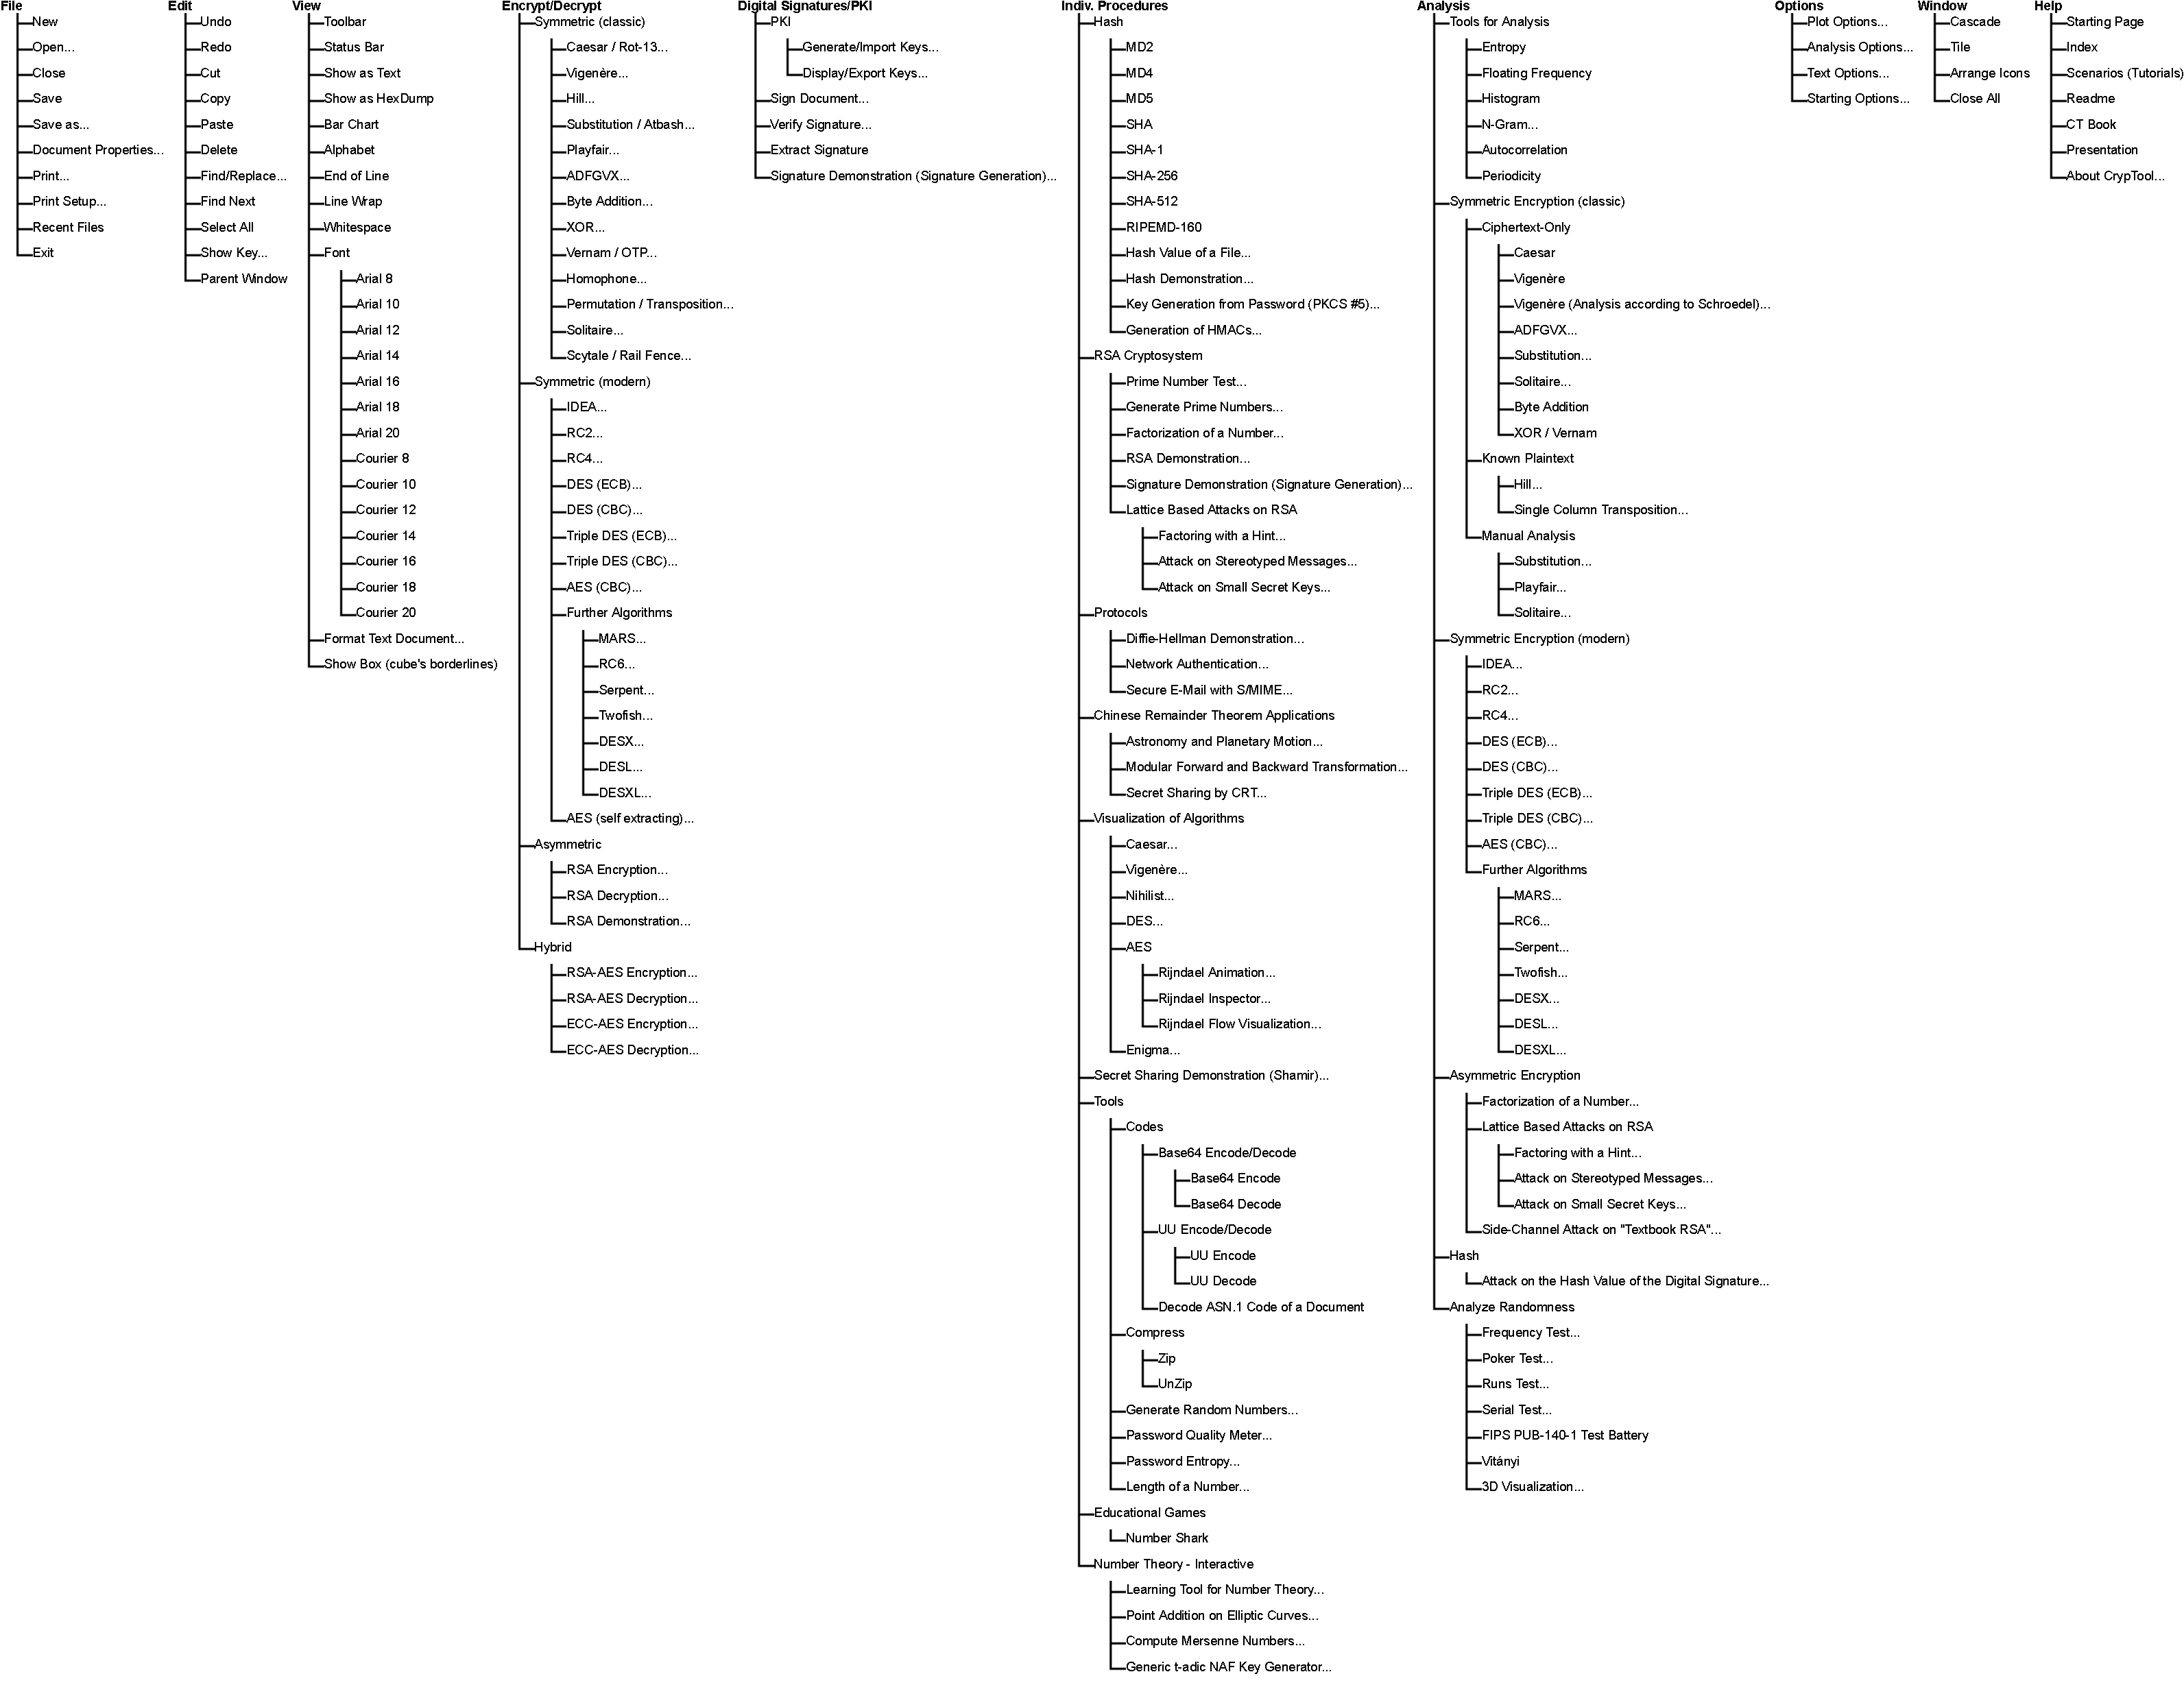
\includegraphics[scale=0.4]{figures/CT1-menutree-en}
\hypertarget{appendix-figure-menu-overview-CT1}{}
\setlength{\abovecaptionskip}{5mm}
\caption{Complete overview of the menu tree of CT1 (CrypTool~1.4.31)}
\label{appendix-figure-menu-overview-CT1}
\end{minipage}
}
\end{center}
\end{figure}
\clearpage
\setlength{\hoffset}{0mm}



%--------------------------------------------------------------------
\newpage
%\enlargethispage{1cm}
\hypertarget{appendix-template-overview-CT2}{}
\section{CrypTool~2 Templates}
\label{s:appendix-template-overview-CT2}

\noindent This appendix contains on the following pages the complete tree with
all templates in CT2\index{CT2}.\footnote{%
  You can find further information about CT2 at:
  \url{http://www.cryptool.org/en/ct2-documentation-en}
}

\noindent When you start CT2 it first shows the Startcenter.

%\clearpage
\begin{figure}[hb]
\begin{center}
%\vspace{-30pt}
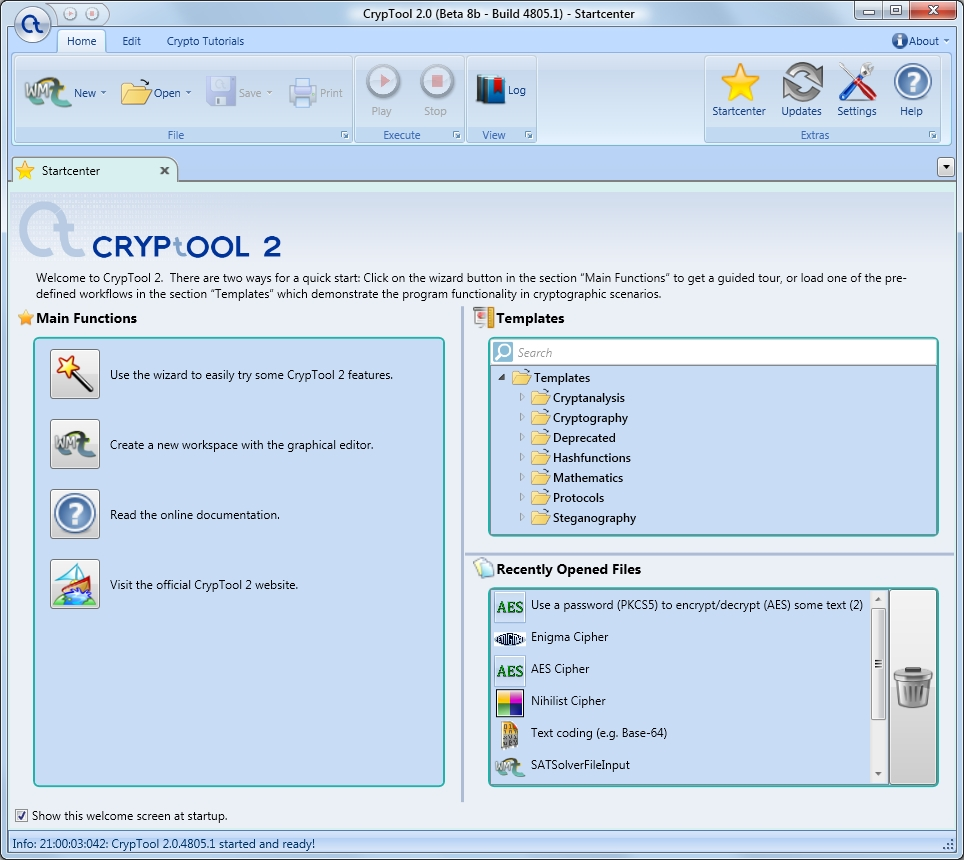
\includegraphics[scale=0.45, angle=0] {figures/CT2-Startcenter-en}
\hypertarget{Welcome-CT2}{}
\caption{Startcenter in CT2 (Beta 8b, May 2012)} 
\label{Welcome-Screenshot-CT2}
\end{center}
\end{figure}
%\clearpage

\noindent Within the Startcenter you have three main ways to use the implemented functionality:
\begin{itemize}
   \item via the Wizard, which leads you to the functions.
   \item via the Workspace, where you can compose the components (e.g. an encryption method, a text input function, ...)  by yourself according to the visual programming\index{visual programming} concept.
   \item via the template tree, which offers ready-to-run workflows.
 \end{itemize}

The Wizard asks questions so you can get to the desired scenarios (e.g. base64 coding) and then runs the according functions. You can afterwards save the chosen scenario as a normal template including the entries you used.

The empty workspace allows to drag on it any component from the navigation bar on the left and connect these components in the way you like. Most of the crypto functionality implemented in CT2 is offered using these components (e.g. Enigma, AES). 

The template tree contains at least one template for each implemented component. The offered templates contain read-to-run workflows. If you change e.g. within the AES template your input, you can see at once, how the output is modified dynamically (e.g. adding another block via padding, influence of the chosen chaining, ...).

\clearpage
\begin{figure}[hb]
\begin{center}
\vspace{-30pt}
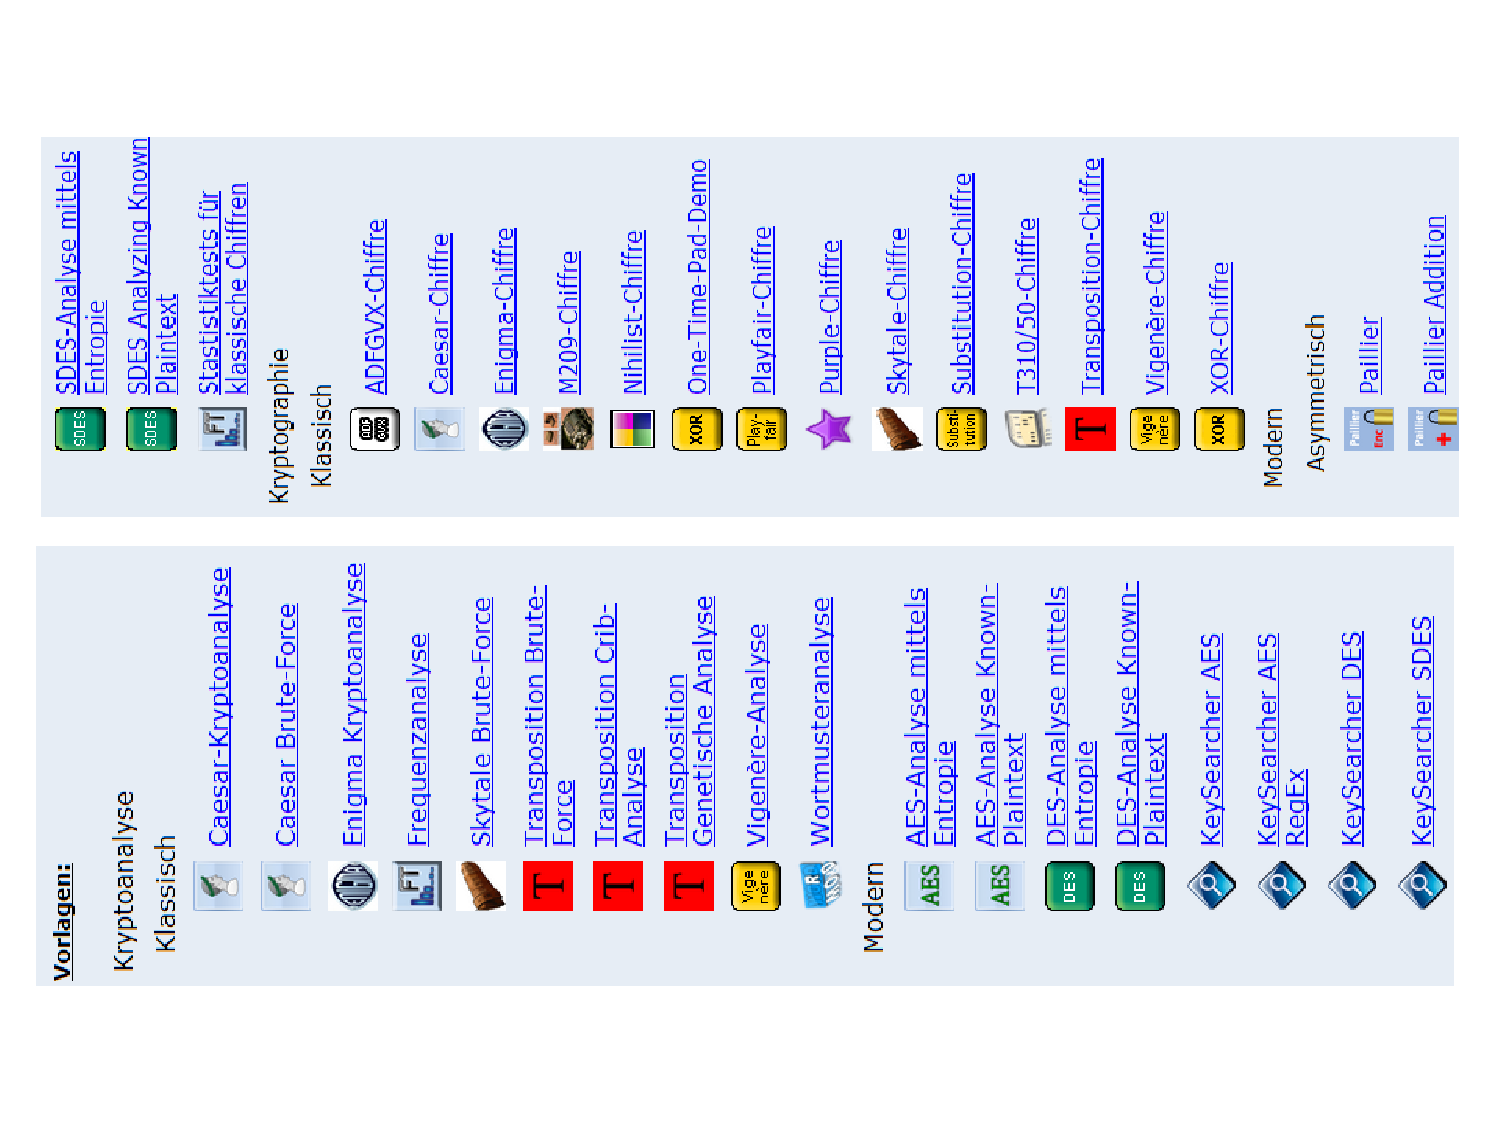
\includegraphics[scale=0.8, angle=270]
                {figures/CT2-templatetree-en-1}
\hypertarget{appendix-figure-template-overview-CT2}{}
\caption{Screenshot of the template tree of CT2 (NB4882.1, July 2012), Part 1} 
\label{appendix-figure-template-overview-CT2}
\end{center}
\end{figure}
\clearpage





%--------------------------------------------------------------------
\newpage
%\enlargethispage{1cm}
\hypertarget{appendix-function-overview-JCT}{}
\section{JCrypTool Functions}
\label{s:appendix-function-overview-JCT}

\noindent On the following pages this appendix contains a list of all
functions in JCrypTool\index{JCT}.\footnote{%
  You can find further information about JCT at:
  \url{http://www.cryptool.org/en/jct-volunteer-en} \\
  This list was generated using the CT Portal website.}

\noindent When you start JCT the first time it shows the Welcome window.

%\clearpage
\begin{figure}[hb]
\begin{center}
%\vspace{-30pt}
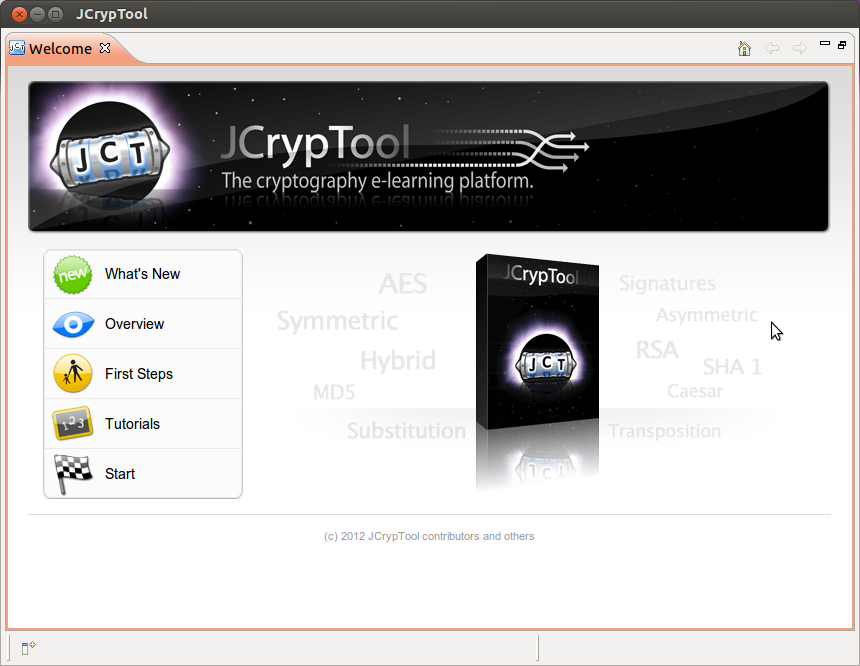
\includegraphics[scale=0.45, angle=0] {figures/JCT-Welcome-EN}
\hypertarget{Welcome-Screenshot-JCT}{}
\caption{Welcome screenshot in JCT (RC6, July 2012)} 
\label{Welcome-Screenshot-JCT}
\end{center}
\end{figure}
%\clearpage
After pressing ``Start'' you can directly use the different functions.
The functions implemented in JCT are presented in two different perspectives:
\begin{itemize}
   \item Default Perspective
   \item Algorithm Perspective
 \end{itemize}

All functions of the {\bf Default Perspective} can be found both in the menus and
in the navigation bar called ``Crypto Explorer'' (at the right side).
The Default Perspective contains all important methods like classic transposition
or modern AES, and many visualizations (e.g. Diffie-Hellman key exchange or
calculations on elliptic curves).

All functions of the {\bf Algorithm Perspective} can be found in the navigation bar
called ``Algorithms'' (in this perspective also at the right side).
The Algorithm Perspective contains all detail settings of the various algorithms, it
especially offers post-quantum computing algorithms\index{post-quantum computing} (PQC).

\clearpage
\begin{figure}[hb]
\begin{center}
\vspace{-30pt}
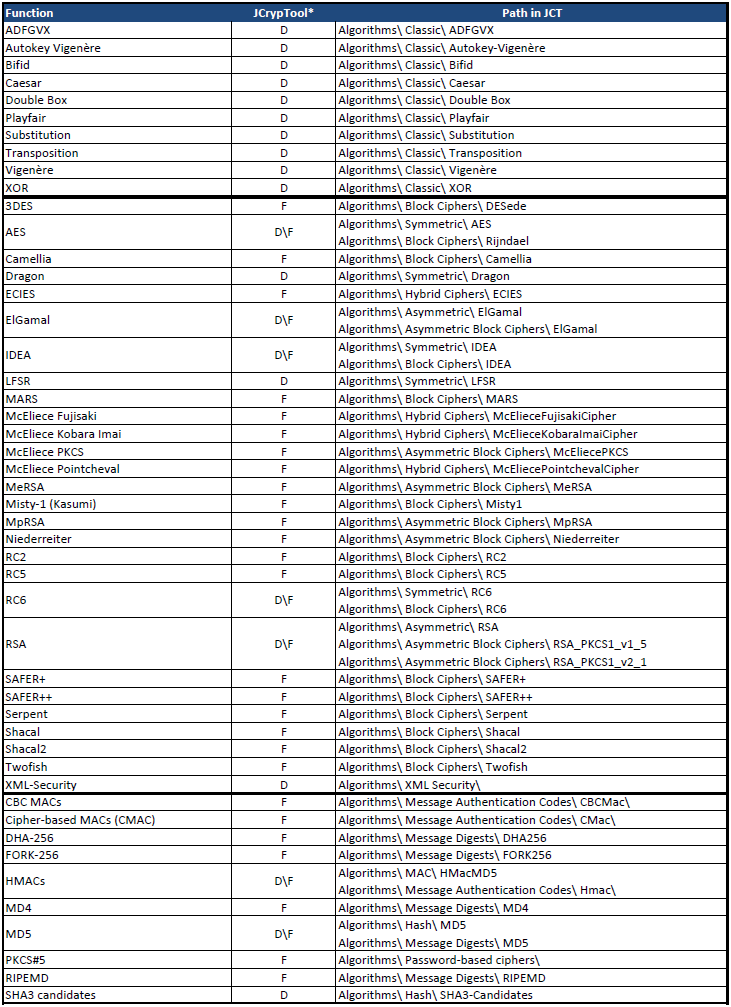
\includegraphics[scale=0.8, angle=0] {figures/JCT-functions-en-1}
\hypertarget{functions-overview-1-JCT}{}
\caption{Screenshot of the functions of JCT (RC6, July 2012), Part 1} 
\label{functions-overview-1-JCT}
\end{center}
\end{figure}
\clearpage

\clearpage
\begin{figure}[hb]
\begin{center}
\vspace{-30pt}
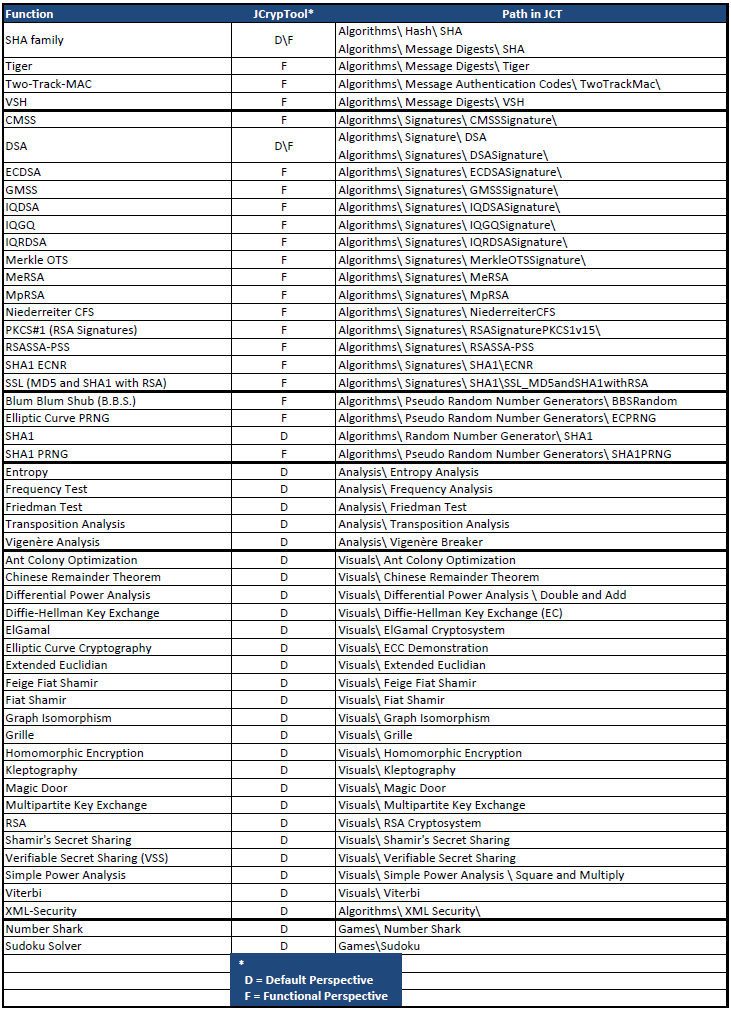
\includegraphics[scale=0.8, angle=0] {figures/JCT-functions-en-2}
\hypertarget{functions-overview-2-JCT}{}
\caption{Screenshot of the functions of JCT (RC6, July 2012), Part 2} 
\label{functions-overview-2-JCT}
\end{center}
\end{figure}
\clearpage





%--------------------------------------------------------------------
\newpage
%\enlargethispage{1cm}
\hypertarget{appendix-function-overview-CTO}{}
\section{CrypTool-Online Functions}
\label{s:appendix-function-overview-CTO}

\noindent This appendix contains a list of all
functions in CrypTool-Online (CTO)\index{CTO}.\footnote{%
  You can find further information about CTO at:
  \url{www.cryptool-online.org} \\
  This list was generated using the functions list at the CT Portal website:\\
  \url{http://www.cryptool.org/ctp-documentation-en/ctp-functions-en}}


%\noindent The starting page of CTO looks like this:
%\begin{figure}[hb]
%\begin{center}
%\vspace{-30pt}
%\includegraphics[scale=0.45, angle=0] {figures/CTO-Welcome-EN}
%\hypertarget{Welcome-Screenshot-CTO}{}
%\caption{Welcome screenshot in CrypTool-Online (November 2012)} 
%\label{Welcome-Screenshot-CTO}
%\end{center}
%\end{figure}


\noindent The following screenshot shows the crypto functions implemented on CTO:
\clearpage
\begin{figure}[hb]
\begin{center}
\vspace{-30pt}
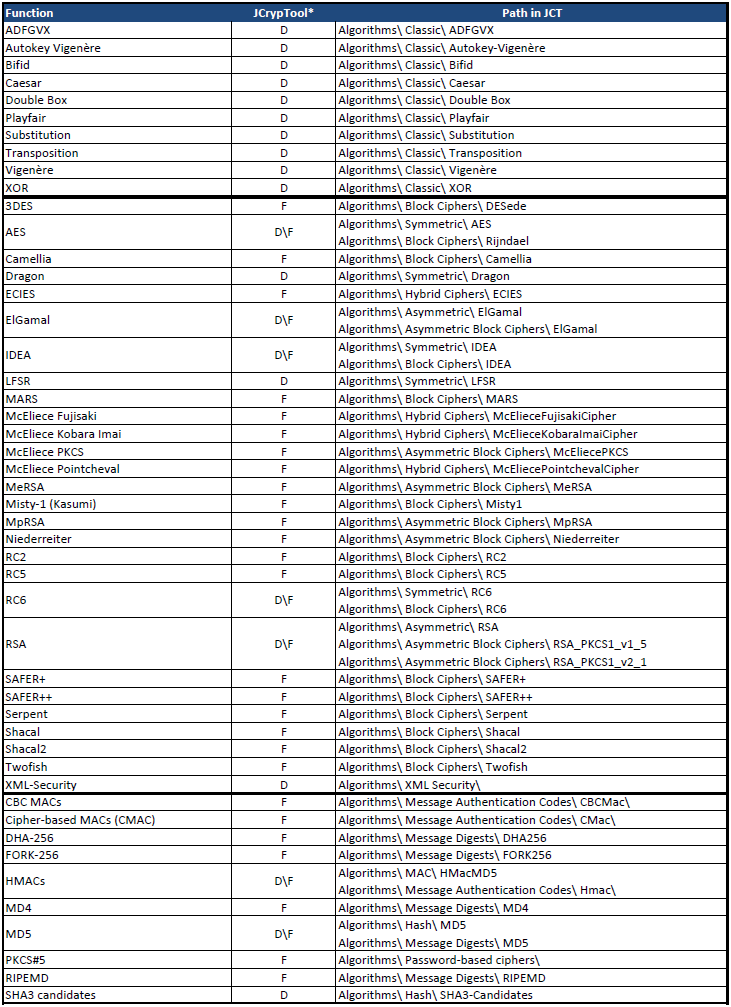
\includegraphics[scale=0.8, angle=0] {figures/JCT-functions-en-1}
\hypertarget{functions-overview-1-CTO}{}
\caption{Screenshot of the functions of CTO (November 2012)} 
\label{functions-overview-1-CTO}
\end{center}
\end{figure}
\clearpage

%\clearpage
%\begin{figure}[hb]
%\begin{center}
%\vspace{-30pt}
%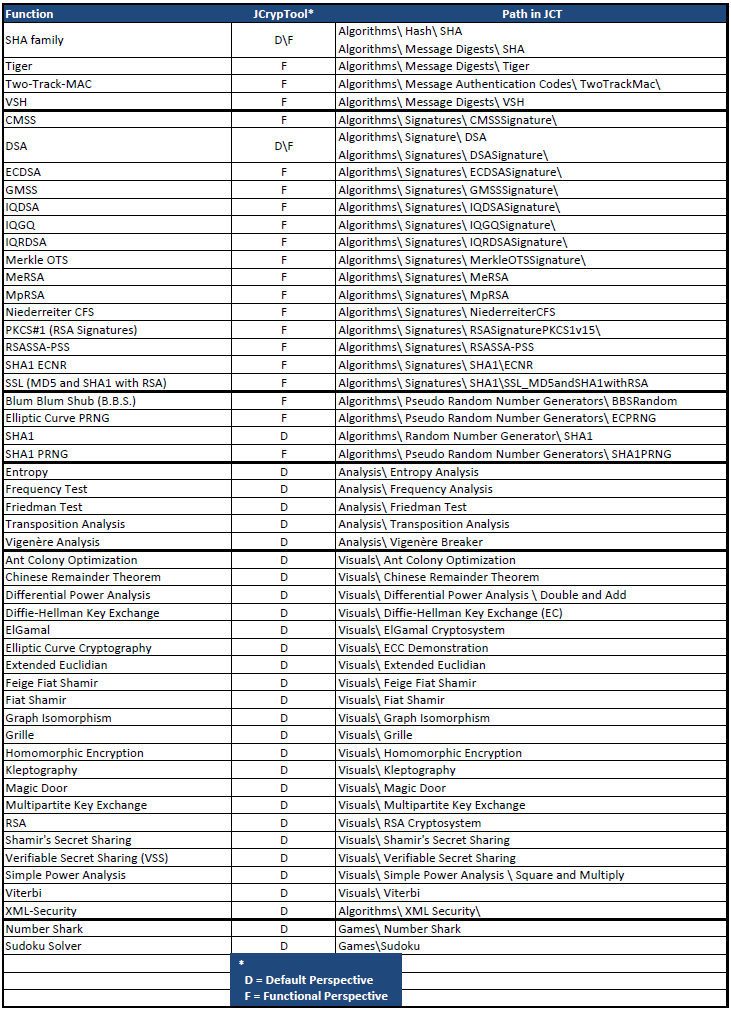
\includegraphics[scale=0.8, angle=0] {figures/JCT-functions-en-2}
%\hypertarget{functions-overview-2-CTO}{}
%\caption{Screenshot of the functions of CTO (November 2012), Part 2} 
%\label{functions-overview-2-CTO}
%\end{center}
%\end{figure}
%\clearpage

